%% LaTeX_Thesis_Template.tex
% An unofficial LaTeX template for Cranfield theses.
% 2017/08/14 Daniel Auger's unofficial Cranfield thesis .sty file
% 2023/05/31 Updated by Shaun Forth (SAF) for logo inclusion
% 2023/06/08 SAF removed capitalisation on title pages on advice of Amy 
% Greenaway and Alison Waters. Added Daniel Auger's headers with 
% chapter and section names.
% 2023/06/08 SAF simplified logo inclusion
% 2026/06/04 Stephanie Burrows (SJB) updated content to bring in line with May 2026 update of CU thesis template
% 2026/06/11 Stephanie Burrows (SJB) updated some features for accessibility

%%
% This document is an example of the use of the "CUThesis2026" 
% LaTeX style file.  

% Document metadata for accessibility
\DocumentMetadata{tagging=on,
    tagging-setup={math/setup=mathml-SE},
    pdfstandard=ua-2,
    pdfstandard=a-4f,
    lang=en-UK
}

\documentclass[12pt,oneside]{book} % for one-sided printing
%\documentclass[12pt,twoside]{book} % for two-sided printing


% Use the custom "CUThesis2026" LaTeX style file. 
\usepackage{CUThesis2026}
\usepackage{lscape} % for landscape pages
% Uncomment the following line (and the relevant \bibliographystyle{} line) to use APA referencing
%\usepackage{apacite} % for APA style referencing - you also need to change the bibliography style

% By default, LaTeX uses a serif font - these are traditionally thought to be
% easier to read.  The following line makes the text sans-serif, which is 
% recommended in the Cranfield Thesis Template. If you'd prefer to use a serif font
% please comment out the following line.
\renewcommand{\familydefault}{\sfdefault}

% Example parameters for a typical taught MSc course 
	\title{My MSc Thesis Title}
	\author{Another Student}
	\date{August 2026}
	\faculty{\FEAS}
	\course{Defence Simulation and Modelling}
	\degree{MSc}
      \supervisor{Dr First A. Supervisor}
	\academicyear{2024--2026}
	\copyrightyear{2026}
		
% Example parameters for a typical PhD
%	\title{My PhD Thesis Title}
%	\author{A. Student}
%	\date{August 2025}
%	\faculty{\FBAM}
%	\degree{PhD}
%	\academicyear{2022--2025}
%	\supervisors{Dr Shaun A. Forth, Dr A. N. Other}
%	\copyrightyear{2025}
%	\copyrightholder{Cranfield University} % for a self-funded PhD, this may be removed
%                                                                    % but many PhD students will be required to 
%                                                                    % assign copyright to others
%	\fulfilment{} % removes message about partial fulfilment
% 

% Logos
% \setCUTextLogo % uncomment to set CU as text on title pages
% \setCUPartnerLogo{PartnerLogo}{Partner's Logo} % uncomment to set joint CU and Partner logos on title 
% pages and you must supply a PartnerLogo.[png,jpg,pdf,...] graphics file for the Partner Logo
%
% Supervisors
% Single supervisor - Use \supervisor
%\supervisor{Dr First A. Supervisor}
% Multiple Supervisors,  use \supervisors. 
%\supervisors{Dr First A. Supervisor and Prof Second Supervisor}
% Associate supervisor use \associatesupervisor
%\associatesupervisor{Dr Associate Supervisor}
% Multiple associate supervisor use \associatesupervisors
%\associatesupervisors{Dr Associate Supervisor and\\ Prof. Yet Another Supervisor}


	

%% COPYRIGHT NOTICES
%
% By default, a Cranfield University copyright statement is displayed. 
% MOD sponsored student theses will usually be Crown Copyright, and 
% should use the following command:
%
%	\copyrightholder{Crown Copyright}
%
% Do something similar if your copyright belongs to anyone else

% Signposting to guidance surrounding intellectual property and copyright ownership 
% can be removed from the cover page by removing or commenting the following lines.
	\copyrightinstructions{(NB. Please refer to the \href{https://www.cranfield.ac.uk/-/
	media/files/rio/research-related-policies/intellectual-property-policy.ashx?la=en&
	hash=A1E0318F44085380F86D3B32BEB1B1FA0532A615}{Intellectual Property Policy}, 
	for full details on intellectual property and copyright ownership; see also guidance in 
	Section~\ref{sec:copyright}.)}

% References



% Cranfield Author Date
%\usepackage{csquotes}
%\usepackage[style=apa]{biblatex}
%\renewcommand{\cite}[2][1]{\parencite[#1]{#2}} % so \cite defaults to \parencite
%\addbibresource{LaTeX.bib}
%\addbibresource{CUCitations.bib}
\includeonly{Author-Date}
 
\begin{document}

%% Front matter
%
% This is where we do the title page, etc.
%

\frontmatter

% Standard-Form Title Pages
\maketitle

% Abstract and Keywords
\begin{abstract}
Replace with your abstract text of not more than 300 words.
\end{abstract}

(NB. If the thesis covers work sponsored by an external body, the name of the sponsor/funding body and the grant number/funding code should be included directly after the abstract.)

\begin{keywords}
Enter at least 6 keywords (not contained within the thesis title).
\end{keywords}

% Acknowledgements
\chapter{Acknowledgements}
This section is not mandatory, but you may wish to acknowledge the support or contributions of other people who have helped with your thesis or with your studies in general.

The author would like to thank Prof. Daniel Auger for his work in previous versions of this template and for testing this version, and Dr Irene Moulitsas and Dr Stephanie Burrows for testing this version.

% Use single spacing for Table of Contents, List of Figures, etc
{
\clearpage
\singlespacing
% Table of Contents
{
\tableofcontents
}
\clearpage

% List of Figures
\listoffigures

\clearpage
% List of Tables
\listoftables
}

% The list of abbreviations can't be automatically generated so you need to populate it yourself
\begin{listofabbreviations}
    \abbrev{FEAS}{Faculty of Engineering and Applied Sciences}
    \abbrev{FBAM}{Faculty of Business and Management}
    \abbrev{STEM}{Science, Technology, Engineering and Mathematics}
\end{listofabbreviations}





%% Main Matter
%
% This is where we include the main thesis content.
%
\mainmatter
\pagestyle{fancy}
\fancyhead[L]{\nouppercase{\leftmark}}
\fancyhead[R]{\nouppercase{\rightmark}}
%\fancyhead[L]{\thetitle}
%\fancyhead[C]{}
%\fancyhead[R]{\theauthor}
%\fancyfoot[L]{}
%\fancyfoot[C]{\thepage}
%\fancyfoot[R]{}

\chapter{Introduction}
\label{sec:Intro}
This guide/template and the associated style file were written to guide Cranfield students in writing a thesis using the \LaTeX\ system so as to closely mimic the University's Microsoft Word Thesis Template available from~\cite{cranfielduniversityTemplatesThesisEnd2026}.

From the Intranet~\cite{cranfielduniversityTemplatesThesisEnd2026} you should be able to download a zip file containing:
\begin{itemize}
\item \texttt{CUThesis2026.sty} - a \LaTeX\ style form that correctly formats your thesis and provides some useful commands.
\item \texttt{CUThesisTemplate2026.tex} - a \LaTeX\ source file used to produce the pdf file you are now reading.
\item \texttt{CULogo.png} - a png image file for the Cranfield logo used on the first two pages of the thesis.
\item \texttt{PartnerLogo.png} -  a sample png image file for a partner organisation.
\item \texttt{FigureExample.png} - a sample image to include in the body of the thesis.
\item \texttt{Latex.bib}, \texttt{CU-Templates.bib} and \texttt{CU-Referencing.bib} - three BibTeX \linebreak source files containing bibliographic data for the citations I have made in this document.
\end{itemize}

Minor guidance content modifications were completed in June 2026 by Dr Stephanie Burrows.

The most recent major version of the template and style file have been tested as follows:
\begin{itemize}
\item the author, using the \LaTeX\ package \texttt{texlive} 2024~\cite{texusersgroupTeXLive2025} updated in January 2025 under Windows 64.
\item Prof. Daniel Auger and Dr Stephanie Burrows using MiKTeX/TeXworks \cite{schenkMiKTeXProjectPage2023} installation on a Cran\-field-main\-tained Windows PC
\item Dr Irene Moulitsas on MacOS using 3 different environments:
	\begin{itemize}
	\item TexShop 5.48 (latest 2025) \cite{kockTeXShop2024}
	\item TeXworks 0.6.9 (latest 2024) \cite{schenkMiKTeXProjectPage2023}
	\item TeX Live 1.54 (circa 2023) \cite{texusersgroupTeXLive2025}
	\end{itemize}
\end{itemize}

\section{Instructions}
\label{sec:Instructions}
I would recommend:
\begin{enumerate}
\item Downloading and unzipping the zip file from the Intranet~\cite{cranfielduniversityTemplatesThesisEnd2026}.
\item  Copy the folder and contents to a new folder (so you keep the original and this document).
\item In the new folder, compiling the template as follows:
\begin{verbatim}
pdflatex CUThesisTemplate2026
bibtex CUThesisTemplate2026
pdflatex CUThesisTemplate2026
pdflatex CUThesisTemplate2026
\end{verbatim}
This should recreate this pdf document you are reading.
\item You should now be able to start editing the document to become your own thesis.
\item If above fails seek help from a colleague or your supervisor who know more about \LaTeX\ than you! 
\end{enumerate}

\begin{flushright}
Shaun Forth $22^{\rm nd}$ January 2025. \\
Minor updates by Stephanie Burrows $11^{\rm th}$ June 2026.
\end{flushright}


 
\chapter{Guidance}
\label{chap:Guidance}
You may wish to save a copy of the template document with this guidance intact for ease of reference. You can also find this guidance and links to training and support resources on the \href{https://cranfield.sharepoint.com/sites/Digital-Skills/SitePages/Thesis-EPA-templates.aspx}{digital skills hub}.

\section{Formatting requirements for your thesis}\label{sec:FormattingRequirements}

\subsection{Mandatory formatting requirements}\label{sec:MandatoryFormatting}
The following requirements are mandatory for the formatting of your thesis. They are built into this template.
\begin{itemize}
\item 3cm margins on all four sides. 
\item Page numbers and any headers or footers should appear within the set margin areas in the template.
\item Any font is acceptable, as long as it is clear and legible. A sans-serif font is recommended. See comments near the beginning of this file for instructions on how to switch to a serif font, if desired.
\item The main body of the text must be 12pt in size, but captions can be smaller, and headings can be larger.
\item Pages must be numbered consecutively. If you wish, you can use Roman numerals for the introductory pages which precede the first chapter.
\end{itemize}

\subsection{Recommended formatting requirements}\label{sec:RecommendedFormatting}
\begin{itemize}
\item Standard A4 printer paper is advised.
\item 1.5 spacing is easier for your examiner to read.
\item There is no requirement to use running headers or footers for chapter headings or for the thesis title, but you may do so if you wish.
\end{itemize}

\section{Basic Document Structure using \LaTeX\ }\label{sec:DocumentStructure}
\subsection{Chapters}
For Chapter Titles use \verb#\chapter{chapter title}# and add an optional\linebreak \verb#\label{label_name}# for ease of referencing. For example, I have inserted\linebreak \verb#\label{chap:Guidance}# for easy cross-referencing to \refChap{chap:Guidance} (using\linebreak \verb#\refChap{chap:Guidance}#) as I shall explain in \refsec{sec:ReferringToHeadings}.  

My use of label names, such as \verb#chap:Guidance# (and later \verb#sec:SectionHeading#, \linebreak \verb#fig:FigureExample#, \etc), is personal preference. The \verb#chap:#, \verb#sec:#, \verb#fig:#, \etc\ prefix just make the labels for chapters, sections, \etc\ easier to find when searching the \LaTeX\ file. 

Try to get in the habit of inserting labels for chapters, sections, \etc, by default. 

\subsection{Section heading}
\label{sec:SectionHeading}
For section headings use \verb#\section{section name}# and add an optional \linebreak\verb#\label{label_name}# for easy cross referencing. \eg \verb#\label{sec:SectionHeading}#.

\subsection{Subsection heading}
\label{sec:SubsectionHeading}
For subsection headings use \verb#\section{subsection name}# and add an optional \linebreak\verb#\label{label name}# for easy cross referencing. \eg \verb#{sec:SubsectionHeading}#.

\subsection{Subsubsection heading}
\label{sec:SubsubsectionHeading}
For subsubsection headings use \verb#\section{subsubsection name}# and add an optional \linebreak\verb#\label{label name}# for easy cross referencing. \eg \verb#{sec:SubsubsectionHeading}#.

\subsection{Referring to headings}
\label{sec:ReferringToHeadings}
Avoid referring to other parts of your document using phases such as ``{\em as described below}'' (unless on the same page, this could be anywhere in the rest of the thesis) or ``{\em as described previously}''  (this could be anywhere from the start of the thesis to this point). Instead make use of the chapter and section labels to point the reader directly to the appropriate part of the thesis. This is called {\em cross-referencing}.

Command \verb#\refchap{label name}# has been defined to make it easy to cross-refer\-ence chapters. Similarly, \verb#\refsec{label name}# is used to cross-reference section, subsection and subsubsection numbers. These commands should be used  when the cross-reference occurs mid-sentence to facilitate their abbreviation. For example, to produce
\begin{quote}
In \refchap{chap:Guidance} we provide guidance on formatting your thesis including, in \refsec{sec:SectionHeading}, section headings. 
\end{quote}
use:
\begin{verbatim}
In \refchap{chap:Guidance} we provide guidance on formatting your 
thesis including, in \refsec{sec:SectionHeading}, section headings. 
\end{verbatim}

At the start of sentences use commands \verb#\refChap{label name}# and\linebreak \verb#\refSec{label name}# to ensure abbreviations for Chapter and Section are not used. For example,
\begin{quote}
\refChap{chap:Guidance} provides guidance on formatting your thesis. \refSec{sec:SectionHeading} covers section headings. 
\end{quote}
is produced using
\begin{verbatim}
\refChap{chap:Guidance} provides guidance on formatting your thesis. 
\refSec{sec:SectionHeading} covers section headings. 
\end{verbatim}
At the time of writing, \verb#\refChap# and \verb#\refchap# produce the same output, but both are included for completeness and in case guidance changes in the future.

\section{Chapter and Section Page Breaks}
\label{sec:ChapSecBreaks}
Use of the \verb#\chapter# command will automatically start a new page. Use of \verb#\section#, \verb#\subsection#  and \verb#\subsubsection# will not. If a page break is desired for improved formatting (\eg a section title appears as the last line on a page and its text appears on the next), then use \verb#\pagebreak# to force a new page where you need it.  

\section{The Title Pages}
\label{sec:TitlePages}
The two title pages and the {\em Academic Integrity Declaration} are created using the \linebreak\verb#\maketitle# command.  However, information for the title pages is \textbf{set in the preamble} (before \verb#\make{document}#) using various commands. Title, author and date are set  using the standard \LaTeX\ commands \verb#\title#, \verb#\author# and \verb#\date#. Other commands are included by \verb#CUThesis2026.sty# as we now detail.

\subsection{Supervisors}
\label{sec:Supervisor}
If there is a single supervisor (plus one or more associate supervisors - see \refsec{sec:AssociateSupervisor}) then use \verb#\supervisor#,
\begin{verbatim}
\supervisor{Dr First A. Supervisor}
\end{verbatim}
But, if there are two or more then use \verb#\supervisors# with appropriate use of {\tt and}, commas, or \verb#\\# (for a line break)  to separate them,
\begin{verbatim}
\supervisors{Dr First A. Supervisor and Prof Second Supervisor}
\end{verbatim}
or,
\begin{verbatim}
\supervisors{Dr First A. Supervisor, Prof Second Supervisor\\ 
and Third Supervisor}
\end{verbatim}
You must set either the supervisor or supervisors. 

\subsection{Associate Supervisors}
\label{sec:AssociateSupervisor}
If there is a single associate supervior then use \verb#\associatesupervisor#,
\begin{verbatim}
\associatesupervisor{Dr Associate Supervisor}
\end{verbatim}
But, if there are two or more then use \verb#\associatesupervisors# with appropriate use of {\tt and}, commas, or \verb#\\# (for a line break)  to separate them,
\begin{verbatim}
\associatesupervisors{Dr Associate Supervisor and Prof. Yet Another}
\end{verbatim}
If you do not set the associate supervisor(s) then nothing is displayed.

\subsection{Faculty}
\label{sec:Faculty} 
Use command \verb#\faculty# to set your Cranfield Faculty of study. There are predefined commands for both of our two faculties. So you might use:
	\begin{itemize}
	\item \verb#\FEAS# for the \FEAS, 
	\item \verb#\FBAM# for the \FBAM.
	\end{itemize}
The obsolete school command, \eg
\begin{verbatim}
\school{\CDS}
\end{verbatim}
should not be used, but will insert the appropriate faculty.

\subsection{Course}
\label{sec:Course}
Taught course students should use the command \verb#\course# to set their course title. \eg
\begin{verbatim}
\course{Defence Simulation and Modelling}
\end{verbatim}
Research students should not set the course (if the course is not set then no course title is written). Please \textbf{do not} set an empty course (\verb#\course{}#) as this causes a \LaTeX\ error that I don't have the time or energy to eliminate.

\subsection{Degree}
\label{sec:degree}
Command \verb#\degree# is used to set your degree of study. 

For taught programmes \cite{cranfielduniversityTaughtDegrees2023} this should be one of 
\begin{itemize}
\item MSc
\item MBA
\item MTech
\item MRes
\item MDes
\item PgDip
\item PgCert
\end{itemize}
For research programmes \cite{cranfielduniversityResearchDegrees2023} this should be one of 
\begin{itemize}
\item PhD
\item Executive DBA
\item EngD
\item MPhil
\item MSc by Research
\end{itemize}
For example,
\begin{verbatim}
\degree{MSc}
\end{verbatim}

\subsection{Academic Year}
\label{sec:AcademicYear}
Aside from the usual \verb#\date# which should be used to supply the month and year of your thesis submission, you should also use \verb#\academicyear# to supply the academic year. For example,
\begin{verbatim} 
\academicyear{2022--2023}
\end{verbatim}



\subsection{Fulfilment}
\label{sec:Fulfilment}
By default the statement,
\begin{quote} 
This thesis is submitted in partial fulfilment of the requirements for the degree of ...
\end{quote}
is added to the second title page. This should be removed for degrees assessed entirely by the thesis, such as a PhD, by using the command,
\begin{verbatim}
\fulfilment{}
\end{verbatim}
in the preamble. 

\subsection{The Cranfield University logo and co-branding}
It is preferred that the Cranfield University logo is positioned at the top of the cover and title pages of the thesis document. The logo image files is provided as \verb#CULogo.png# with this template and included by default. (It can also be specified using the command \verb#\setCULogo#.)

If it is not appropriate to show the Cranfield University logo, then it can be removed and replaced by the text as described in \refsec{sec:UseCUText}.

If you are working with a partner on the research included in this thesis document, you may, subject to their approval, also include their official logo as co-branding on the cover and title pages. Guidance is provided in \refsec{sec:UsePartnerLogo}.



\subsection{Using Cranfield University text in place of a logo}
\label{sec:UseCUText}
If appropriate you may remove the Cranfield University logo from the cover and title pages of the thesis and in its place use the text “CRANFIELD UNIVERSITY”.

To remove the Cranfield logo issue the command
\begin{verbatim}
\setCUTextLogo
\end{verbatim}






\subsection{Adding a partner logo}
\label{sec:UsePartnerLogo}
Before using a partner logo in this document you must:
\begin{itemize}
\item obtain permission from the partner to use their logo in this document.
\item obtain a high-resolution logo from the organisation – do not take a screen-shot from the website.
\end{itemize}
To add the partner logo as co-branding use
\begin{verbatim}
\setCUPartnerLogo{PartnerLogo}{Partner's Logo}
\end{verbatim}
where \verb#PartnerLogo.png# or \verb#PartnerLogo.jpg# is the graphics file containing your partner's logo. A dummy \verb#PartnerLogo.png# is supplied with this template. The text ``Partner's Logo'' is used as alternative text for a screenreader, to enable accessibility.

The Partner Logo is automatically scaled to be the same width as the CU Logo. This might not be appropriate if the logo is wider than tall. In that case experiment with the command \verb#\setCUPartnerLogo# in the style file \verb#CUThesis2026.sty#. You may wish to consult~\cite{carlisleCTANPackageGraphicx2021,thelatexprojectteamCTANPackageArray2024} for support in doing so.

\section{Copyright}
\label{sec:copyright}
For further details on the intellectual property and copyright ownership, please refer to the  \href{https://www.cranfield.ac.uk/-/media/files/rio/research-related-policies/intellectual-property-policy.ashx?la=en&hash=A1E0318F44085380F86D3B32BEB1B1FA0532A615}{Intellectual Property Policy}, CU-RIO-POL-5.0,  Section 2 and Section 5. 

MOD-sponsored student theses will usually be Crown Copyright and should include the copyright statement below (Section 5 of the Intellectual Property Policy refers).
\begin{quote}
\textbf{\copyright\ Crown Copyright, 20XX. All rights reserved. No part of this publication may be reproduced without the written permission of the copyright holder.}
\end{quote}
Students sponsored by other employers or funders may also have different copyright statements.

\subsection{Assigning Copyright within the \LaTeX\ thesis template}
By default, only the year is displayed, as copyright remains with the student, who is the author of the document. The copyright year must be supplied: this will be the same as the year of submission. For example,
\begin{verbatim} 
\copyrightyear{2023}
\end{verbatim}
A different copyright holder can be specified as follows:
\begin{itemize}
\item For MOD-sponsored students:
\begin{verbatim}
\copyrightholder{Crown Copyright}
\end{verbatim}
\item To assign copyright to Cranfield University:
\begin{verbatim}
\copyrightholder{Cranfield University}
\end{verbatim}
\item Other copyright holders may be assigned in a similar way.
\end{itemize}
Please note that instructional text has been added to the cover page regarding intellectual property and copyright ownership. This may be removed from the cover page by commenting out the line beginning
\begin{verbatim}
\copyrightinstructions
\end{verbatim}
near the beginning of the \texttt{CUThesisTemplate2026.tex} document.

\section{Inserting captions in the main document}
Captions should be used whenever you insert a graphic or table. Use the \verb#\caption# command to create the caption and add a \verb#\label# for cross-referencing. 

\subsection{Figures - graphs, photos, diagrams}
A \LaTeX\ \verb#\figure# environment should be used to insert graphs, photos and diagrams - here I'm also using them for \LaTeX\ code listings (an alternative would be to set up a new environment for listings and use a better \LaTeX\ package for displaying it \cite{schopfCTANPackageVerbatim2024,vanzandtCTANPackageFancyvrb2024,hoffmanCTANPackageListings2024}). The caption should be placed below the figure. An example is shown in \reffig{fig:FigureExample}.
\begin{figure}[ht]
\begin{center}
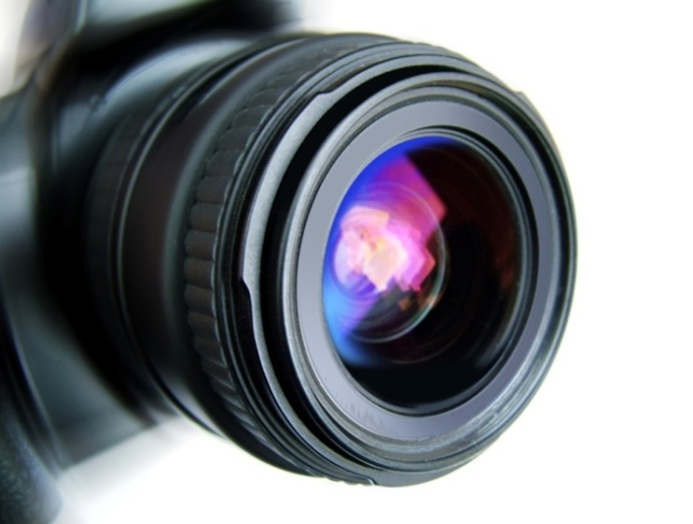
\includegraphics[width=0.8\textwidth,alt={A photograph of a camera, used as an example for the template.}]{FigureExample}
\end{center}
\caption{A figure caption}
\label{fig:FigureExample}
\end{figure}  
This was coded using the following:
\begin{verbatim}
\begin{figure}[ht]
\begin{center}
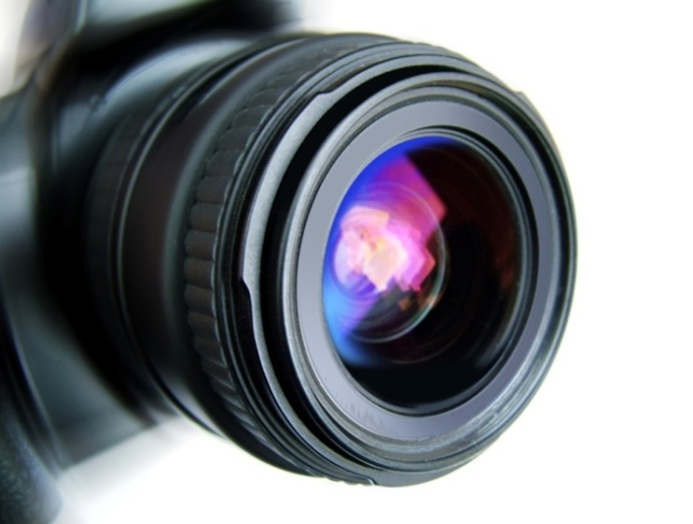
\includegraphics[width=0.8\textwidth,
	alt={A photograph of a camera, used as an example for the template.}]
	{FigureExample}
\end{center}
\caption{A figure caption}
\label{fig:FigureExample}
\end{figure}  
\end{verbatim}
Note the figure placement options \verb#[ht]# to place the figure as best as possible either (h=) here (at the place where coded) or at the (t=) top of the page. Otherwise it will be placed on the following page. 

Please use \texttt{alt} to include alt-text, which provides a description of the image for the screenreader. This enables the creation of an accessible document.

If you wish to include sub-figures, that is two or more graphs, phots or diagrams alongside each other with the same main caption then consider using the subfigure package~\cite{bidi-texgithuborganisationCTANPackageSubfig2005}

\subsection{Tables}
A \LaTeX\ \verb#\table# environment should be used to insert tables, with the table itself generated using the \verb#\tabular# environment.  An example is shown in \reftab{tab:TableExample}.
\begin{table}[ht]
\caption{A table caption}
\begin{center}
\tagpdfsetup{table/header-rows={1}}
\begin{tabular}{l|l|l}
& Heading & Heading \\ \hline
Label & Detail & Detail \\
Label & Detail & Detail \\ \hline
\end{tabular}
\end{center}
\label{tab:TableExample}
\end{table}
The caption should be placed above the table. The coding to achieve this is:
\begin{verbatim}
\begin{table}[ht]
\caption{A table caption}
\begin{center}
\tagpdfsetup{table/header-rows={1}}
\begin{tabular}{l|l|l}
& Heading & Heading \\ \hline
Label & Detail & Detail \\
Label & Detail & Detail \\ \hline
\end{tabular}
\end{center}
\label{tab:TableExample}
\end{table}
\end{verbatim}
The 
\begin{verbatim}
\tagpdfsetup{table/header-rows={1}}} 
\end{verbatim}
command provides accessibility support so that the table is appropriately interpreted by the screenreader.

\subsection{Equations}
Equations with labels are easily coded in \LaTeX\ using the \verb#\equation#  environment and  \verb#\label# command,
\begin{equation}
A=\pi r^2. \label{eq:circlearea}
\end{equation}
This is coded as
\begin{verbatim}
\begin{equation}
A=\pi r^2. \label{eq:circlearea}
\end{equation}
\end{verbatim}
Remember to punctuate your equation with a period if it ends a sentence. 

Equations should only be labelled if they are cross-referenced later. Use \verb#\[.\]# for an unlabelled equation,
\[
A=\pi r^2.
\]

For derivations it is often useful to use the \verb#eqnarray# environment. For example, multiplying out a quadratic,
\begin{eqnarray}
y&=&(x-3)(x+4) \nonumber\\
&=& x^{2}+x-12 \label{eq:quadratic}
\end{eqnarray}
with \verb#\nonumber# used to label constituent equations that do not need labelling. This is coded as 
\begin{verbatim}
\begin{eqnarray}
y&=&(x-3)(x+4) \nonumber\\
&=& x^{2}+x-12 \label{eq:quadratic}
\end{eqnarray}
\end{verbatim}

\subsection{Referring to captions for figures, tables etc.}
We can reference figures, tables and equations using supplied \verb#\refFig#, \verb#\reffig#, \linebreak\verb#\refTab#, \verb#\reftab#, \verb#\refEqn# or \verb#\refeqn# according to what we are referencing, and whether we are doing so at the start of a sentence or not. Here are some examples:
\begin{itemize}
\item \refTab{tab:TableExample} at start of a sentence
\begin{verbatim}
\refTab{tab:TableExample} at start of a sentence 
\end{verbatim}
\item Within sentence reference to \reftab{tab:TableExample} 
\begin{verbatim}
\item Within sentence reference to \reftab{tab:TableExample} 
\end{verbatim}
\item \refEqn{eq:quadratic} at start of a sentence
\begin{verbatim}
 \refEqn{eq:quadratic} at start of a sentence
\end{verbatim}
\item Within sentence reference to \refeqn{eq:quadratic} 
\begin{verbatim}
\item Within sentence reference to \refeqn{eq:quadratic} 
\end{verbatim}
\end{itemize}

\subsection{Updating Tables of Contents, Lists of Figures and Labels}
The information for contents, figures, tables and labels and cross-referencing for \LaTeX\ are enabled using various files: \verb#.toc# (table of contents), \verb#.lof# (list of figures), \verb#.lot# (list of tables)\verb#.aux# file. \Eg for this \LaTeX\ file \verb#LaTeX_Thesis_Template.toc#,\linebreak \verb#LaTeX_Thesis_Template.lof#, \verb#LaTeX_Thesis_Template.lot# and \linebreak \verb#LaTeX_Thesis_Template.aux# are created. The labels, captions, \etc\  are written to these files when a command such as \verb#\chapter# or \verb#\label# during processing of the \LaTeX\ file (\eg when running \verb#pdflatex#).   The labels, chapter names, \etc\ are also read from this file to generate the table of contents, list of tables, and cross-references. As a result you will need to process the file at least twice to get the table of contents, list of tables and cross-references correctly updated.

Sometimes these files may get corrupted if the labels, chapter names etc are not correctly coded. In this case you will need to remove the \verb#.toc# (table of contents), \verb#.lof# (list of figures), \verb#.lot# (list of tables)\verb#.aux# files. There is often a simple menu option to do this if using \LaTeX\ through a GUI tool such as \verb#TeXworks# for which the drop down {\em File -- Remove Aux Files ...} may be used.

\begin{landscape}
\section{Inserting Landsape Pages}
It is often preferable to use a landscape page to display tables of data, charts or diagrams.  
\begin{figure}[ht]
\begin{center}
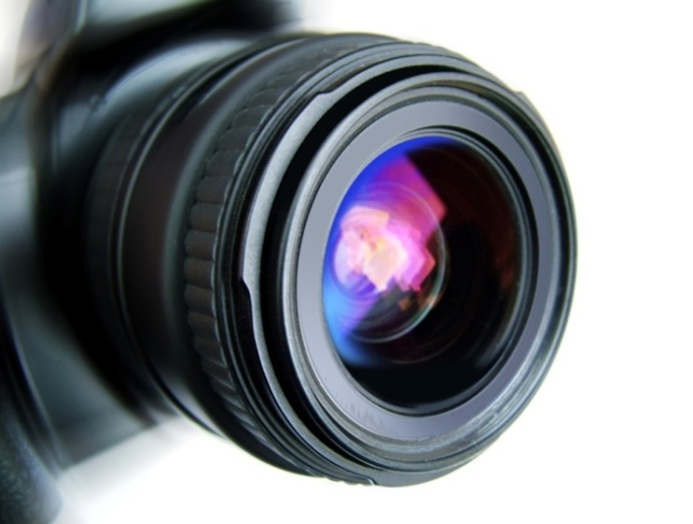
\includegraphics[width=0.8\textwidth,alt={A photograph of a camera, used as an example for the template.}]{FigureExample}
\end{center}
\caption{A figure on a rotated page caption}
\label{fig:FigureExampleRotated}
\end{figure} 
\end{landscape}
This is most easily done by using the \verb#lscape# package~\cite{carlisleCTANPackageLscape2020} and placing the \LaTeX\ source for the content to be created with the \verb#landscape# environment. 
\begin{verbatim}
% preamble
% : 
\usepackage{lscape}
% 
\begin{document}
% :
\begin{landscape}
% source for landscape material
\end{landscape}
\end{verbatim}


\chapter{Referencing}
\label{chap:referencing}
The University specifies that you should use the APA7 Author-Date \cite{cranfieldlibraryserviceAPA7AuthorDateReferencing2024} or the Cranfield Numbered \cite{cranfielduniversitylibraryservicesNLMNumberedReferencing2023} citation styles as advised by your course director or supervisor. 

You may wish to do your own research into choosing an appropriate bibliography style and how to use this within \LaTeX, but just as a start, guidance for switching to the APA referencing style is provided.

Essentially, you need to uncomment the following line in the preamble of this document:
\begin{verbatim}
\usepackage{apacite}
\end{verbatim}
and then swap the bibliography style in the reference section to the following:
\begin{verbatim}
\bibliographystyle{apacite}
\end{verbatim}
Be aware that you will likely need to remove all of the ``Aux Files'' (all the additional files that are created along with the final PDF document) in the current folder in order to get this to compile properly. It may not be enough to use the \texttt{Remove Aux Files...} option from within the file menu within TeXworks (if this is what you're using) - you may well need to manually remove all of these files and start compilation from scratch.

Generally we only include {\em References} (books, articles, \etc we have referenced in the body of the thesis) in scientific and engineering theses. If you also need a {\em bibliography} (books, articles, \etc, useful in your background research but unreferenced in the body of the thesis) then you'll need to research this and report back to me! 

\section{Guidelines for referencing potentially sensitive information}\label{sec:SensitiveInformation}
Consider whether documents you are using could potentially contain commercially sensitive information. If in doubt always check with the source organisation (or its successor, if it is no longer in existence) on what you can do with them; and where you do want to use them, what conditions the document owner wishes to apply.

If you are involved in classified research it is important that you don’t cite documents without first checking whether they can be referenced. If they are referenced you must ensure that the classification of your own thesis should be at least at the same security level. If you have any doubt or concern about citing a source, please check with your supervisor and/or Library staff.

%\section{Cranfield APA7 Author-Date Referencing}
\label{sec:authordaterefs}
Ensure the following lines are uncommented in the preamble to the template file
\begin{verbatim}
SHAUN ADD
\end{verbatim}
and towards the end of the file
\begin{verbatim}
SHAUN ADD
\end{verbatim}

We now cover a few of the examples from the APA7 Author-Date \cite{cranfield_library_service_apa7_2021}. 

\subsection{Journal Articles}
\label{sec:NumberedJournal}
\begin{description}
\item[Journal article with one author and no DOI]:
\begin{description}
\item[Parenthetical citation:] A recent article discussed the fracture... \parencite{hutchinson_fracture_2010}.
\item[Narrative citation:] Recently, \textcite{hutchinson_fracture_2010} discussed the fracture ...
\end{description}

\item[Journal article with two authors]:
\begin{description}
\item[Parenthetical citation:] It was not possible to separate targets \parencite{yang_perceptual_2016}.
\item[Narrative citation:]  \textcite{yang_perceptual_2016} found it was not possible to separate targets.
\end{description}

\item[Journal article with three to twenty authors]:
\begin{description}
\item[Parenthetical citation:] Previous authors \parencite{langley_process_2013} have identified assumptions \ldots .
\item[Narrative citation:]  \textcite{langley_process_2013} identify assumptions\ldots .
\end{description}

\item[Journal article with twenty one or more authors]:
If there are twenty-one or more authors, in the reference list add the names of the first nineteen
authors followed by \ldots and then the last author’s name.

\item[Online journal article with DOI] The synthesis of a new polymer of
cadmium(II) \linebreak ethylenediamineazide was determined by \ldots \parencite{yang_preparation_2010}. 
\item[Online journal article with URL] The synthesis of a new polymer of
cadmium(II) \linebreak ethylenediamineazide was determined by \ldots \parencite{yang_another_2010}.
\item[Journal article with no author]  TC-32B QT was demonstrated at an
exhibition held in Kent \cite{anon_first_2005}.
\end{description}

\subsection{Newspaper Articles}
\label{Sec:Newspapers}
If you are citing an online news website, e.g., BBC News, format the reference as a webpage (refer
to the section on the Internet).

\begin{description}
\item[Printed newspaper article] A blast at an atomic weapons factory was
met with denials by Iran \cite{frenkel_europe_nodate}.\\
\textbf{Note:} Use bibtex \texttt{misc} type, omit date from \texttt{year} field and place date in \texttt{note} field. 
\item[Article from an online newspaper]  Rayner \cite{rayner_combat_2011} reports that The Royal British Legion Centre for Blast Injury Studies is
to design…
\end{description}

\subsection{Books}
\label{sec:NumberedBooks}
\begin{description}
\item[Book with a single author] According to \textcite[p.35]{sommerville_software_2007} the most important part of software engineering is…
\item[Book with two authors] \textcite[p.65]{stair_principles_2010} suggest…
\item[Book with four or more authors] This was noted by \textcite[p.15]{payne_relationship_1995}
\item[Book with an editor] Latest thinking on gender in organizations
suggests… \cite{kumra_oxford_2014}
\item[Chapter of an edited book] \textcite[p.35]{haase_standards_2005} identified...
\item[Chapter of an edited book with organisation as author e.g. handbooks] 
The steel corrosion showed …\parencite{asm_international_corrosion_1998}
\item[Book with no author] In order to vote in the UK…\parencite{noauthor_whitakers_2011}
\item[Electronic book (eBook) or an online book] The project manager’s role can be defined as… \parencite{kerzer_project_2009}
\item[Book accessed via an eReader e.g. Kindle, iPad etc.]
Brodie tried to decipher the \linebreak code~\cite{dennis_secret_2012}\\
\textbf{NOTE: Place eReader type in square brackets at the end of the bibtex title field}
\item[Translated Book] In his discussion about algebraic
topology, \textcite[p.17]{matvev_lectures_2006} considered...\\
\textbf{Translator not yet supported}
\end{description}



\subsection{Conference Papers}
\label{sec:NumberedConference}
\textbf{NOTE:} Use bibtex entry \texttt{incollection}.
\begin{description}
\item[Full conference proceeding] The IEEE \cite[p.59]{noauthor_11_2010} suggests that \ldots
\item[Individual paper] \textcite{moon_aeroacoustic_2003} provide computations \ldots\\
\textbf{NOTE:} Place paper number in the bibtex \texttt{number} field.
\item[Online proceeding or paper] \textcite{wessel_assessing_2010} provide a ten step method\ldots
\item[Offshore Technology Conference (OTC) paper] According to \textcite{chiasson_large_1999} large bore \ldots
\end{description}

\subsection{Internet}
\label{sec:Internet}
\textbf{NOTES:} 
\begin{itemize}
\item The bibtex style file does not support the \texttt{accessed} attribute so include it in the note field of the bibtex entry.
\item If using Zotero then use a \texttt{document} and not a \texttt{web} entry as the \texttt{publisher} field is often used
\end{itemize}
\begin{description}
\item[Web page with an individual author] \textcite{bradley_notitle_2011} states that libraries and \ldots
\item[Web page with an organisation as author] The Natural Hazards Centre \cite{university_of_colorado_boulder_natural_2011} advised
that \ldots
\item[Blog] \textcite{borger_afghanistan_2010} claims in `Afghanistan
options are running out' \ldots\\
\textbf{NOTE: add [Blog] to end of title field.}
\item[Wiki] The CILIP ARLG National committee
meeting notes show \ldots \cite{barefoot_october_2012}
\textbf{NOTE: add [Wiki] to end of title field.}
\end{description}

\subsection{Thesis or dissertation}
\label{sec:thesis}
\begin{description}
\item[Print thesis or dissertation] An examination of Forth’s \citeyear{forth_morphological_1989}
research shows that…
\item[Online thesis or dissertation] \textcite{tatham_confidence_2010} identifies three areas
undergoing notable change…\\
\textbf{NOTE: use of question mark in thesis title is not presently detected in bibtex style file.}
\end{description}


\subsection{Course materials}
\label{sec:course}
\begin{description}
\item[Lecture or seminar] The lecture provoked much debate~\cite{johnson_peat_2012}
\item[Lecturers’ notes on Virtual Learning Environment \eg\ Canvas] As illustrated in the course materials~\cite{forth_analysis_2012}
\item[Course Virtual Learning Environment discussion forum] The debate during the lecture continued in the discussion forum. \textcite{hurst_are_2012} was
particularly vociferous.
\end{description}

\subsection{Official Publications}
\label{sec:officialPubs}
\textbf{Note:} These have not been tested yet but can probably be achieved with a bibtex \verb#misc# entry.
\begin{description}
\item[UK Statute (Act of Parliament)] 
\item[House of Commons or House of Lords Paper]
\item[House of Commons or House of Lords Bill]
\item[Statutory Instruments (SIs)]
\item[Hansard Debate]
\item[Command Paper (Green or White Paper)]
\item[European Directive]
\end{description}

\subsection{Reports}
\label{sec:Reports}
\begin{description}
\item[Report] An analysis of China’s investment in companies in different countries has shown... \cite{wolf_chinas_2011}.
\item[Online report] The effect was… \cite{curry_-flight_1989}.\\
\textbf{Note:} Presently unable to get colon (:) between report number and report title.
\item[Online industry or market research report] Media trends in the UK…\cite{marketline_media_2013}
\item[Online company or annual report] Despite economic uncertainty the
company’s profits did increase \cite{rolls-royce_group_plc_annual_2011}.
\item[Online company or financial report or data source] Rolls-Royce plc turnover has dramatically
reduced in 2009-2010 \cite{bureau_van_dijk_rolls-royce_2010}.
\end{description}


\subsection{Case Studies}
\textbf{Note:} These have not been tested yet but can probably be achieved with a bibtex \verb#misc# entry.

\subsection{Working Papers}
\textbf{Note:} These have not been tested yet but can probably be achieved with a bibtex \verb#misc# entry.




\subsection{Standards, patents, protocols and datasheets}
\label{sec:standards}
\textbf{Note:} 
\begin{itemize}
\item Use bibtex \texttt{report} item
\item Presently unable to get colon (:) between report number and report title.
\end{itemize}
\begin{description}
\item[Standard] In projects "specification, schedule and
cost always have to be bounded to ensure
ongoing viability" \cite{british_standards_institution_project_2010}.
\item[Online standard from a database] Some standards provide guidelines for effective project management \cite{british_standards_institution_project_2010}.
\item[Patent] The method of assembly... \cite{hodge_rear_2008}
\item[Joint Service Publication or protocol] The MOD has a simple definition of knowledge \cite{great_britain_ministry_of_defence_retaining_2011}.\\
\textbf{Note:} As the actual url is not available, put the availability and accessed data in the bibtex \texttt{note} field.
\item[Datasheet \eg ESDU] The buckling of the panel… \cite{esdu_elastic_2008}.
\end{description}

\subsection{Datasets and software}
\label{sec:datasets}
\begin{itemize}
\item Use bibtex \texttt{misc} type.
\item Include version number in parenthesis in the \texttt{title} field.
\end{itemize}
\begin{description}
\item[Dataset] Data from \textcite{partridge_spectra_2014} showed \ldots
\item[Software] Plone is an example of this sort of use
of an open source content management
system~\cite{plone_foundation_plone_2016}.
\end{description}

\subsection{Audio visual materials}
\textbf{Note:} These have not been tested yet but can probably be achieved with a bibtex \verb#misc# entry.

\subsection{Images}
\label{sec:images}
\textbf{Notes:} 
\begin{itemize}
\item Use \texttt{misc} type
\item For items available online   so include the \texttt{accessed} attribute in the \texttt{note} field of the bibtex entry.
\end{itemize}
\begin{description}
\item[Illustration, figure, diagram, logo or table] The estimated sales forecast is shown in \reffig{fig:sales}.
\begin{figure}[ht]
\begin{center}
\includegraphics[width=0.6\textwidth]{Sales}
\end{center}
\caption{Estimated Sales Forecast~\parencite[p.4]{wisker_good_2012}}
\label{fig:sales}
\end{figure}
\item[Embedded illustration, cartoon, diagram, etc.] The pressure on the housing market… \cite{wood_cartoon_2014}.\\
\textbf{Note:} Include the \texttt{[medium]} , here a \texttt{[cartoon]} at the start of the bibtex title field.
\item[Ordnance Survey map] P.O. equates to Post Office \parencite{ordnance_survey_oxford_1994}.\\
\textbf{Note:} 
\begin{itemize}
\item Use the \texttt{title} field to add the map number and scale.
\item Use the \texttt{note} field to add the map series.
\end{itemize}
\item[Online map] There are many farms in the area \parencite{ordnance_survey_peak_2010}.\\
\textbf{Note:} The bibtex style file does not support the \texttt{accessed} attribute so include it in the note field of the bibtex entry.
\item[Painting or drawing] \textbf{Note:} This has not been tested yet but can probably be achieved with a bibtex \verb#misc# entry.
\item[Painting or drawing online] Groves’ {\em Carrot on a stick} \citeyear{groves_carrot_2007} is playing with colours. 
\item[Photograph – print or slide] 
Sublime lighting captures the atmosphere
wonderfully \cite{collins_pictures_2010}\\
\textbf{Note:} I uses a \texttt{book} entry here.
\item[Photograph online or in an online collection \eg Flickr, Instagram] An abundance of movement is
captured \cite{rush_running_1997}.
\end{description}


\subsection{Personal communications}
\textbf{Notes:}\\
\begin{itemize}
\item Use \texttt{misc} type
\item If dates are not fully listed then place them in the \texttt{note} field.
\end{itemize}
\begin{description}
\item[Email or letter] The details of the organisational structure
were outlined \cite{godfrey_restructure_nodate}.
\item[Conversation] It was felt the organisational culture
changed when the new CEO arrived \cite{williams_conversation_nodate}.
\item[Interview, survey or questionnaire] The theory was dismissed as
nothing new \cite{benson_should_nodate}.
\end{description}



%\include{Numbered}






\chapter[Dealing with long chapter names]{Dealing with chapters whose 
chapter name is ridiculously long and so spoiling formatting}
Apart from new chapter pages, the style file automatically uses the current chapter and section names for the left and right headers of the pages of the main body. This can cause problems if the chapter or section names are too long. To cope with this, when you define the new chapter, also define a shortened chapter name in square brackets, as we have for this chapter,
\begin{verbatim}
\chapter[Dealing with long chapter names]{Dealing with chapters whose 
chapter name is ridiculously long and so spoiling formatting}
\end{verbatim}
\refSec{sec:longSection} shows how to do this for sections. 

Note that the short chapter and section names are also used in the table of contents so try to avoid long names if possible.

\newpage
\section[Dealing with long section names]{Dealing with sections whose 
section name is ridiculously long and so spoil formatting}
\label{sec:longSection}
Please avoid long section names. If you must have them then it's advisable to provide a short section name
\begin{verbatim}
\section[Dealing with long section names]{Dealing with sections whose 
section name is ridiculously long and so spoil formatting}
\end{verbatim}


\chapter{More Topics}
This is a sample of thesis text. This is a sample of thesis text. This is a 
sample of thesis text. This is a sample of thesis text. This is a sample of
thesis text.

This is a sample of thesis text. This is a sample of thesis text. This is a 
sample of thesis text. This is a sample of thesis text. This is a sample of
thesis text.


\chapter{Final Topic}
This is a sample of thesis text. This is a sample of thesis text. This is a 
sample of thesis text. This is a sample of thesis text. This is a sample of
thesis text.

This is a sample of thesis text. This is a sample of thesis text. This is a 
sample of thesis text. This is a sample of thesis text. This is a sample of
thesis text.


\chapter{Conclusions}
This is a sample of thesis text. This is a sample of thesis text. This is a 
sample of thesis text. This is a sample of thesis text. This is a sample of
thesis text.

This is a sample of thesis text. This is a sample of thesis text. This is a 
sample of thesis text. This is a sample of thesis text. This is a sample of
thesis text.


%% Back matter
%
% This is where we include references and appendices
\renewcommand{\bibname}{References}  % for the report or book class
% Swap the bibliography style to apacite to use APA referencing (you also need to \usepackage{apacite}
% in the preamble)
\bibliographystyle{vancouver}
%\bibliographystyle{apacite} % For APA referencing
\bibliography{LaTeX,CU-Templates,CU-Referencing}

%\printbibliography

\appendix

\chapter{Ethical Approval Letter}\label{app:EthicalApproval}
% Insert your own CURES letter here. The CURES system seems to name the letter ``Letter.pdf'' by default,
% so this might be as simple as just saving this PDF document within your thesis folder (replacing the
% existing Letter.pdf dummy file with your own letter), and compiling your thesis. If necessary, you can 
% adjust the placement of the letter on the page by changing the inputs to the ``trim'' option below -
% these (along with the clip option) trim the margins off the original PDF with the syntax
% ``trim={<left> <bottom> <right> <top>}''. Adjust these as needed for your own document.
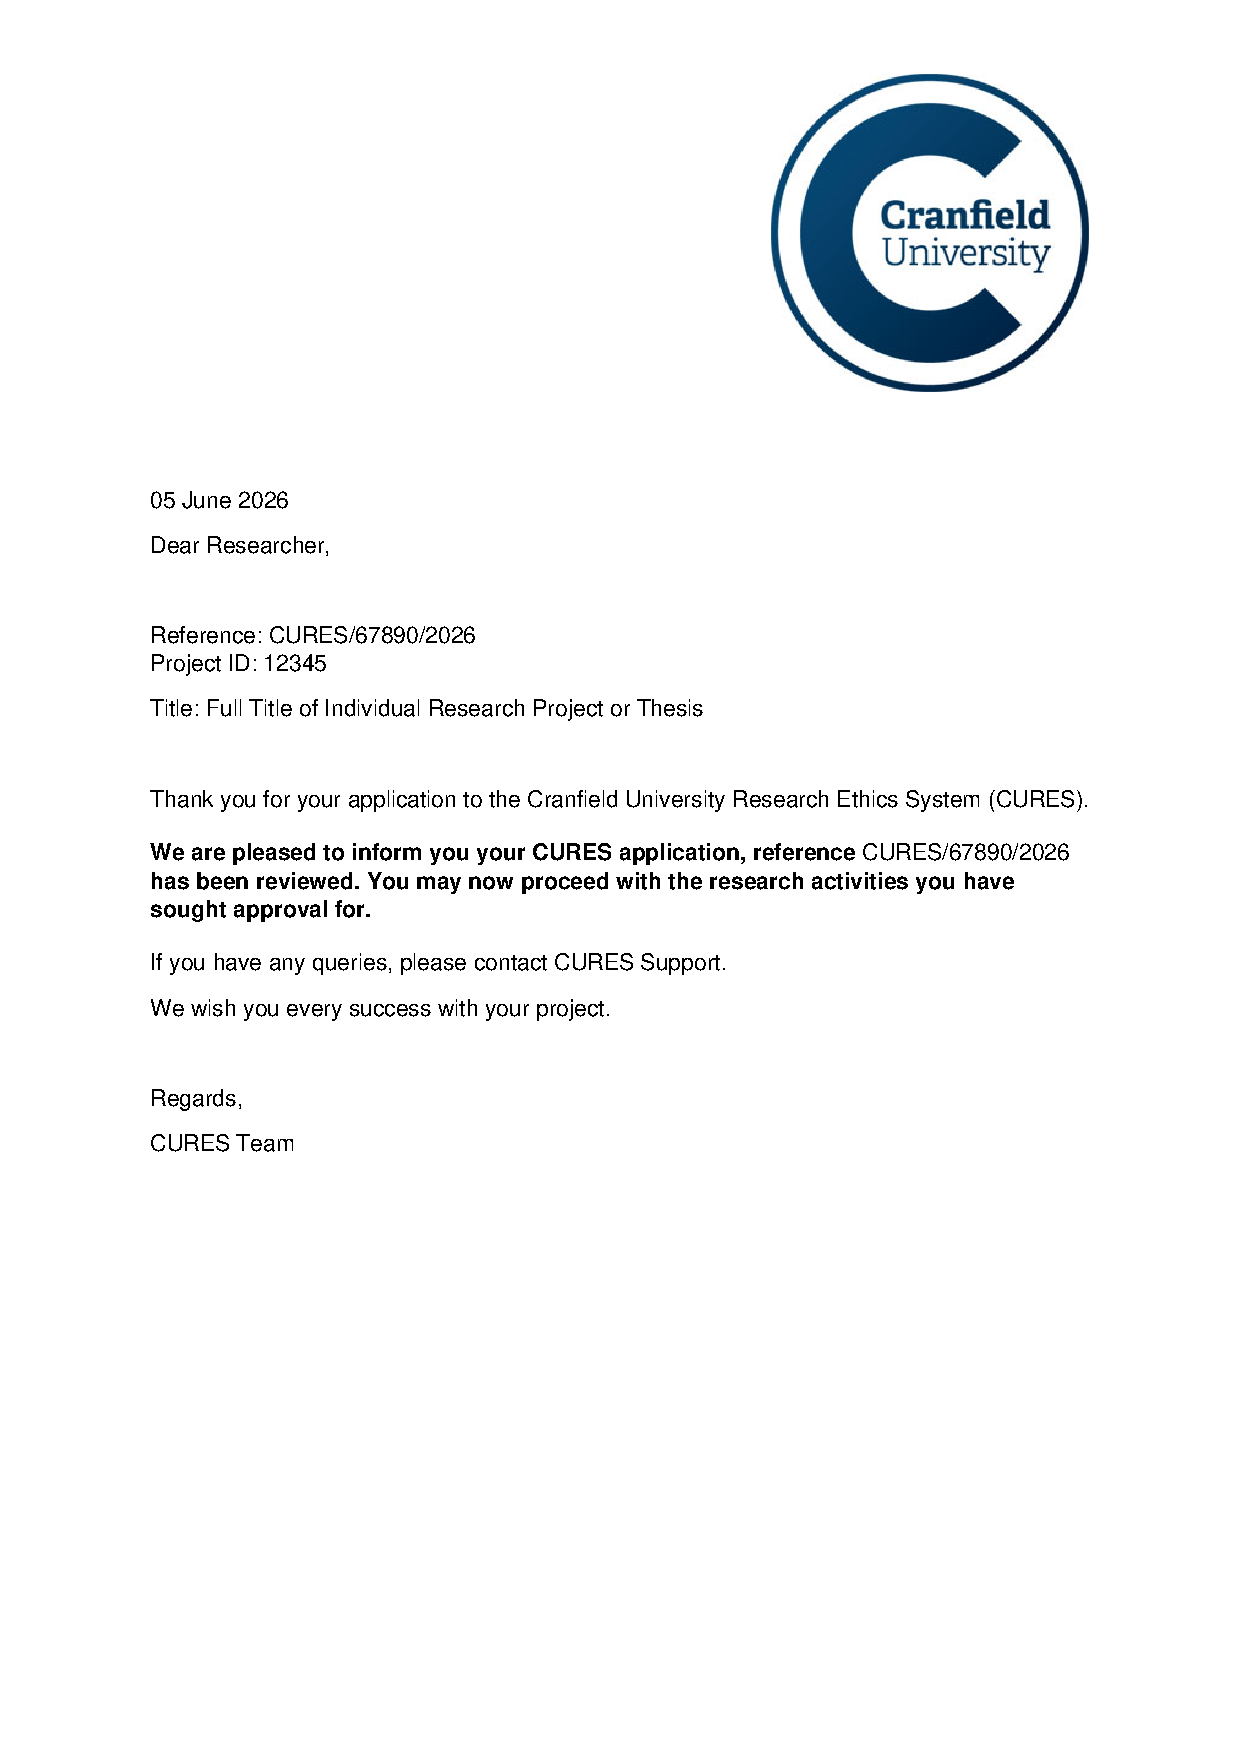
\includegraphics[width=\textwidth, trim={2cm 10cm 2cm 1.25cm}, clip, alt={The ethical approval letter from the CURES system.}]{Letter.pdf}

\chapter{Ethical Approval Guidance}\label{app:EthicalApprovalGuidance}
Insert your ethical approval letter as the first appendix, i.e. Appendix A. The letter is emailed to you following CURES approval.

All research must have appropriate ethical approval before data collection commences.

\section{Taught students}
If you have not gained ethical approval or cannot provide confirmation of ethical approval your thesis will not be marked. This may result in award failure. Non-approval will be escalated to the Research and Innovation Office. This is in accordance with Section 10.2 of the Senate Handbook \href{https://www.cranfield.ac.uk/-/media/files/corporate_documents/managing-taught-courses.ashx?la=en&hash=FA9E8D01D902FABBE036B1AB70A8B7CFF5C3E465}{Managing Postgraduate Taught Courses}.

\section{Research students}
Retraction of thesis - In accordance with section 12.3 of the Senate Handbook \href{https://www.cranfield.ac.uk/-/media/files/corporate_documents/managing-research-students.ashx?la=en&hash=DAB3E4550D9CF9D3FE1605CA5E1F12F055C1FB2A}{Managing Research Students}, exceptionally, a supervisor may hold the view that the quality of the thesis falls considerably short of the required standard, or may have concerns that the thesis does not meet the expected standards relating to ethics or academic integrity. 

In such cases, a supervisor may request that the relevant Director of Research authorises the retraction of a thesis. The Director of Research will, following discussion with the supervisor, review with the research student the issues raised and determine whether the thesis is retracted formally or whether the examiners should be instructed to proceed with the examination arrangements.

\section{Including the letter via \LaTeX}
The letter may be include in the thesis document using the following commands:
\begin{verbatim}
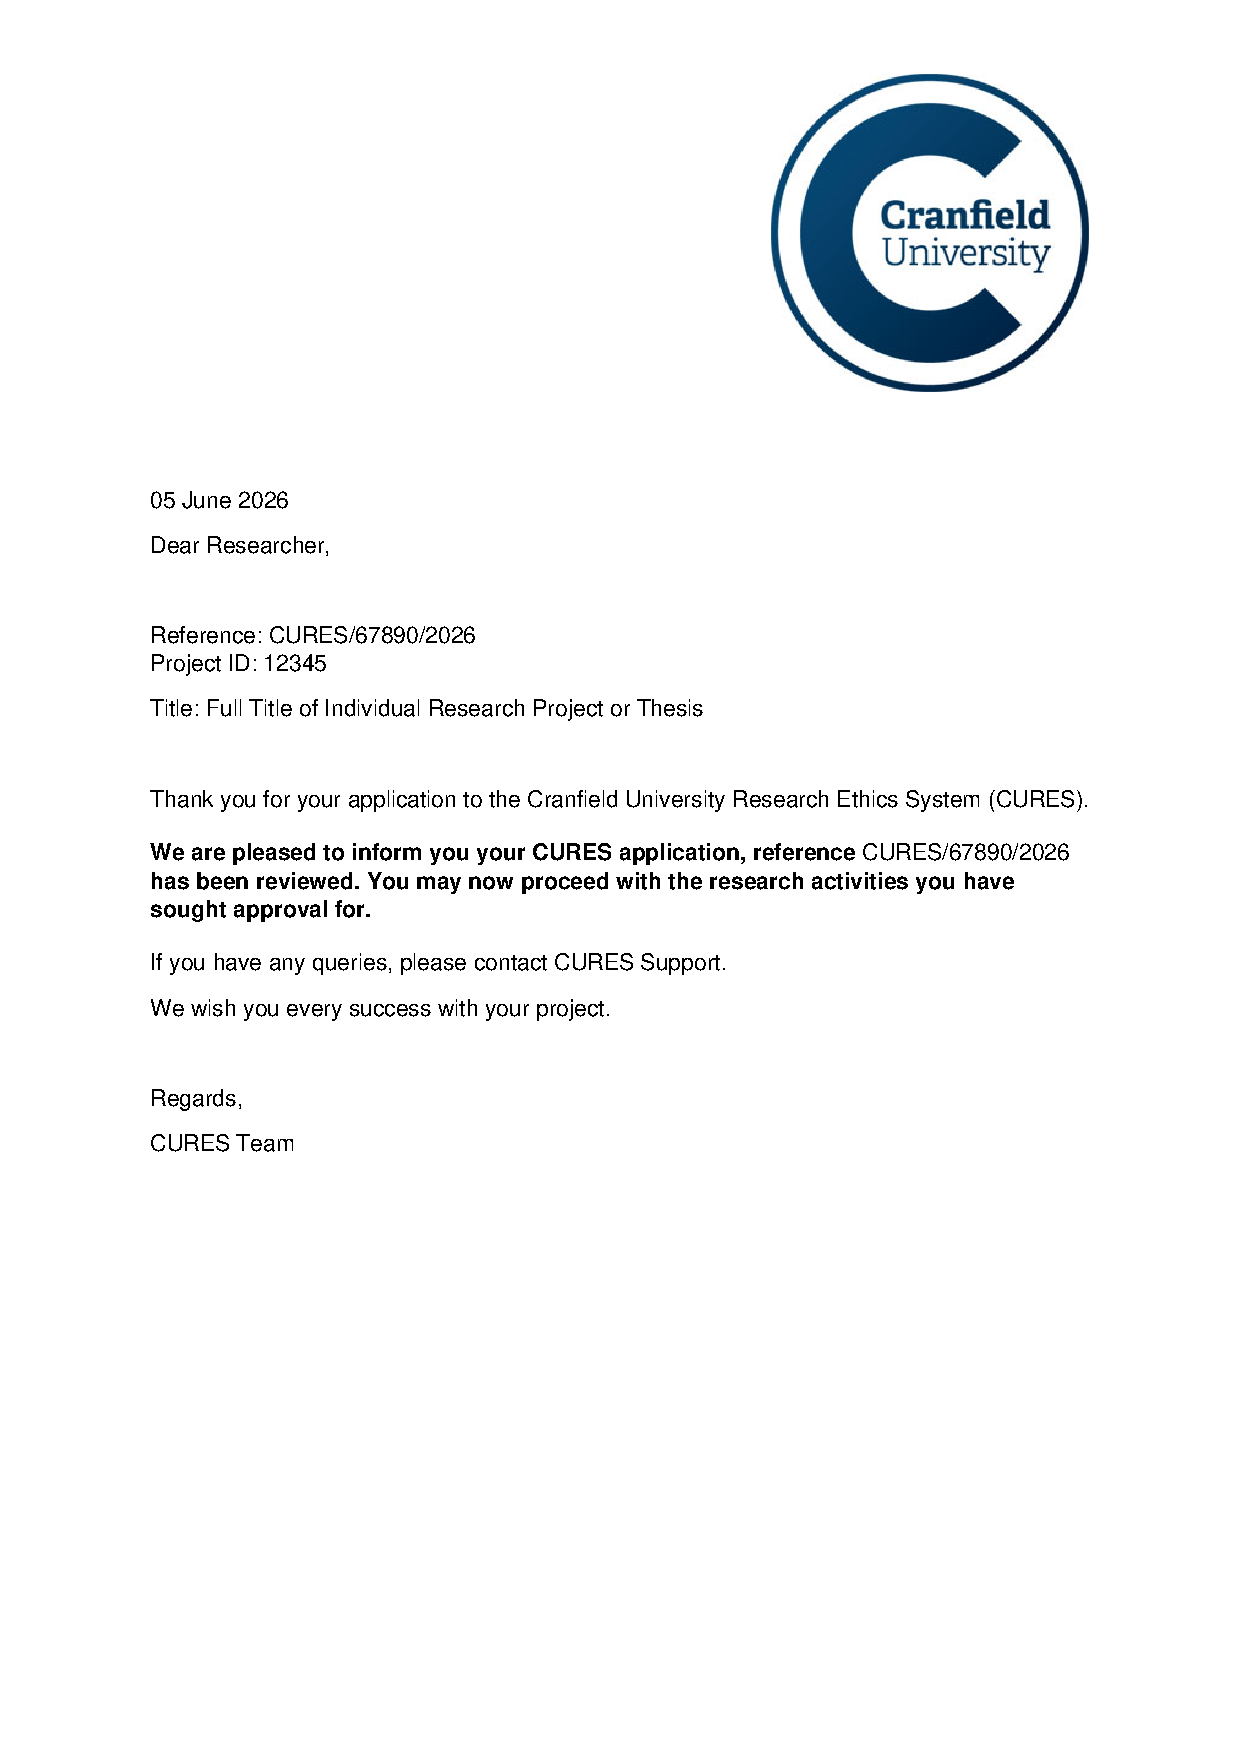
\includegraphics[width=\textwidth, trim={20 300 20 15}, clip,
	alt={The ethical approval letter from the CURES system.}]
	{Letter.pdf}
\end{verbatim}
A placeholder has been placed in Appendix~\ref{app:EthicalApproval}. You can adjust the \texttt{trim} option values to ensure all of the text in the letter is included, without the text becoming too small to read. Suggested values are given for the placeholder, but your letter might vary from this.

\chapter{Extra Data}
This is a sample of thesis text. This is a sample of thesis text. This is a 
sample of thesis text. This is a sample of thesis text. This is a sample of
thesis text.

This is a sample of thesis text. This is a sample of thesis text. This is a 
sample of thesis text. This is a sample of thesis text. This is a sample of
thesis text.





\end{document}

